%%%%%%%%%%%%%%%%%%%%%%%%%%%%%%%%%%%%%%%%%%%%%%%%%%%%%%%%%%%%%%%%%%%%%%%%%%
%
%    JWST_sci_template.tex  (use only for JWST General Observer and Archival Research proposals)
%
%
%
%    JAMES WEBB SPACE TELESCOPE
%    OBSERVING PROPOSAL TEMPLATE
%    FOR CYCLE 1 (2017)
%
%    Version 1.0 September 2017.
%
%    Guidelines and assistance
%    =========================
%     Cycle 1 Announcement Web Page:
%
%         https://jwst-docs.stsci.edu/display/JSP/JWST+Cycle+1+Proposal+Opportunities
%
%    Please contact the JWST Help Desk if you need assistance with any
%    aspect of your proposal:
%    	    http://jwsthelp.stsci.edu
%
%
%
%%%%%%%%%%%%%%%%%%%%%%%%%%%%%%%%%%%%%%%%%%%%%%%%%%%%%%%%%%%%%%%%%%%%%%%%%%%

% The template begins here. Please do not modify the font size from 12 point.

\documentclass[12pt]{article}
\usepackage{jwstproposaltemplate}
\usepackage{hyperref}
\usepackage{graphicx}
\usepackage{floatrow}
\usepackage{sidecap}
\sidecaptionvpos{figure}{t}



\usepackage{natbib}
\bibliographystyle{mnras}

% \usepackage[]{biblatex}
% \addbibresource{WAFLS.bib}
% \addbibresource{WAFLS_quiescent.bib}

\setlength{\textfloatsep}{5pt}
\usepackage{color}

\newcommand{\todo}[1]{\textbf{**TODO: \textcolor{red}{#1}**}}


\begin{document}

%   1. SCIENTIFIC JUSTIFICATION
%       (see https://jwst-docs.stsci.edu/jwst-opportunities-and-policies/jwst-call-for-proposals-for-cycle-1/jwst-cycle-1-proposal-preparation)
%
%






\todo{Abstract. Delete later.}


\todo{Science}

Pure parallel opportunities on \emph{Webb} offer the opportunity, \emph{almost for free}, to build up a large amount of public NIRCam imaging complementing GO programmes. We propose to exploit the longest available opportunities to build up $\sim 150\ {\rm arcmin^2}$ of deep (F200W$=29-29.5$) multi-band NIRCam imaging data. This proposal - the Public Ultradeep Pure Parallel Imaging Extragalactic Survey (PUPPIES) - 

PUPPIES will make modest gains on JADES, increasing the area surveyed at F200W$=29-29.5$ depth by $\sim 20\%$. However the PUPPIES will be immediately public and will result in 




% We propose WAFLS - the Wide Area First Light Survey. WAFLS is a pure-parallel programme designed to build up a large ($\sim 1350$arcmin$^2$) area of medium-depth (F200W=$28.5$) 6-band near-infrared ($1-5\mu$m) imaging with NIRCam. WAFLS complements planned GTO and ERS programmes by obtaining shallower imaging over an area $4-5\times$ larger (comparable to {\it HST}'s CANDELS survey), separated into $\sim$150 independent pointings, minimising the effect of cosmic variance. The primary scientific motivation of WAFLS is the identification and characterisation of the $L^{\star}$ galaxies at $9<z<11$ including placing strong constraints on the bright-end of the luminosity function. The multi-wavelength observations observations obtained by WAFLS will enable the accurate measurement of key physical properties of these galaxies including the star formation rate, morphologies, dust attenuation, and stellar masses. The sources identified by WAFLS will be more amenable to multi-wavelength follow-up with other facilities. The secondary motivation is the selection of high-$z$ passive (i.e. non star-forming) galaxy candidates and the analysis of their abundance at $3<z<6$. The large area observed by WAFLS will be key to identify such sources, rare yet crucial to constrain the physical mechanisms responsible for their rapid assembly and efficient star formation suppression in the early Universe.  Compared to JADES (CEERS), WAFLS will include ~5x (~10x) more quiescent galaxies at $z>3$.  




\clearpage

\justification          % Do not delete this command.


\todo{Opening statement about important of the early Universe}

The past near-decade of wide and deep surveys with the {\it Hubble Space Telescope’s} ({\it HST}) Wide Field Camera 3 (WFC3) has begun the process of exploration of this key epoch in the Universe’s history.  Wide and deep surveys with WFC3 over the Hubble Ultra Deep Field (HUDF; Beckwith et al. 2006; Bouwens et al.\ 2010; DUNLOP+), Cosmic Assembly Near-Infrared Deep Extragalactic Legacy Survey (CANDELS; Grogin et al.\ 2011; Koekemoer et al.\ 2011), and the Frontier Fields project (REFERENCE) enabled the construction of the first large samples of galaxies at $z>7$.  Among the discoveries made with these data are 1) While the faint-end slope of the UV luminosity function steepens significantly at $z>7$, the bright-end shows less evolution (e.g., Bouwens et al.\ 2015; Finkelstein et al.\ 2015); 2) The abundance of galaxies, when integrated to very faint limits now provided seemingly feasible from lensing studies (e.g., Atek et al.\ 2015; Livermore et al.\ 2017) imply that galaxies produce enough photons to complete reionization by $z\sim$ 6, though only if the ionizing photon escape fraction is $\gtrsim$10\% (REFERENCES); 3) Bright/massive galaxies appear modestly dusty, showing an early onset of chemical enrichment (Finkelstein et al.\ 2012; Bouwens et al.\ 2014, UPDATE REFERENCES), and 4) Bright/massive galaxies exist out to at least $z \sim$ 10 (e.g. Oesch et al.\ 2016).

Little is known however about the galaxy population at $z>9$ beyond the discovery of a few candidate galaxies.  While some studies of the evolution of the galaxy population imply a dramatic decline in the UV luminosity density (and by extension, star-formation rate density) at $z >$ 9 (e.g., Bouwens et al.\ 2015; Oesch et al.\ 2018), others see no such decline (e.g., Coe et al.\ 2013; McLeod et al.\ 2016), and the discovery of an unexpectedly luminous galaxy at $z >$ 10 (Oesch et al.\ 2016) points towards potentially significant amounts of star-formation activity remaining to be discovered in this epoch of galaxy formation.  Predictions from simulations also span a wide range (see left-panel of Fig. 4), but those that attempt to account for the evolution of the physical conditions promoting star formation, most notably the dependence of star-formation rate on gas density, predict again {\it Webb}-detectable levels of star-formation at $z >$ 9 (e.g., Yung et al.\ 2018).  A key question for the opening cycles of {\it Webb} is this — is there significant star-formation activity at  $9<z<12$, or does the limiting redshift of {\it HST} just happen to coincide with the time when the universe began its first large-scale episode of star formation?


While the planned GTO/ERS programmes, in particular the Cosmic Evolution Early Release Science (CEERS) and the JWST Advanced Deep Survey (JADES), will begin the process of obtaining stronger constraints at $z>9$. However, the expected 

and while JADES is expected to yield more, observations will be spread over the first 3 cycles, with the full data-set potentially not becoming public until 4 years after launch. 

To address this we propose to exploit pure parallel opportunities to rapidly build up a large area of very-deep F200W$>29$ public multi-band NIRCam imaging. 

Our programme



\noindent
\textbf{The primary scientific objectives of WAFLS are:}
\vspace{-1mm}
\begin{enumerate}
\item The robust identification of tens of bright (F200W$<28$) galaxies across the early EoR ($9<z<11$) amenable to multi-wavelength follow-up.
\item Cosmic variance minimised constraints on the $9<z<11$ luminosity function around $L^{\star}$.
\item The measurement of the physical properties of $9<z<11$ galaxies including their star formation rates, stellar masses, dust attenuation, and morphologies. 
\item Constraints on the space density and properties of quiescent galaxies at $z>3$ including the first useful constraints at $z>5$.
\end{enumerate}

While focused on the distant Universe WAFLS will provide an invaluable immediately public legacy resource for answering a range of other science questions. WAFLS will, for example, enable the discovery and typing of low-mass stars and sub-stellar objects throughout the disk and halo of the Milky Way. When combined with optical observations WAFLS will enable the measurement of accurate stellar masses and star formation rates across cosmic history, reaching down to $M_{\star}\sim 10^{8}\,{\rm M_{\odot}}$ at $z=2$.


\subsection*{Constraints on the UV Luminosity Function Across the Epoch of Reionisation and Beyond}\label{sec:UVLF}



% THIS TEXT IS TAKEN FROM ANOTHER PROPOSAL IN PREP - IT SHARES SOME COIs SO I FEEL ITS FINE AS A REFERENCE

% The first 500 Myr of galaxy evolution (z>10) was a transformative period in our Universe, as the first galaxies began to coalesce, enriching and ionizing their environments, forever altering the course of subsequent gas accretion and star formation. While deep and wide surveys with HST (e.g., HUDF [PI Illingworth], CANDELS [PIs Faber & Ferguson], Hubble Frontier Fields [PI Lotz]) led to the discovery of ∼1000 galaxy candidates at 6< z <8, Hubble has only scratched the surface at z>9, with just a handful of z ∼9–11 tenuous (e.g., <10σ significance in 1–2 imaging bands) candidates [27, 4]. Pushing HST’s limits has led to a tension in published observational results. While there is agreement that the observable (MUV < −17) cosmic SFR density smoothly declines from z = 4 to 8 [e.g., 14, 6], some [e.g., 27] find evidence for an accelerated decline at z > 8, while others [e.g., 25, 12] find evidence for a continued smooth decline to earlier times. The absence of robust observational constraints leaves theoretical models completely unconstrained at z >9 (Figure 2), where differences in their physical star-formation and feedback prescriptions result in a wide range of predictions for the abundance of galaxies during this epoch. This leads to enormous uncertainty on plausible timelines for the reionization of the intergalactic medium (IGM), where models which follow the steep SFR density evolution are consistent with a slow beginning and rapid completetion, while those which follow the shallow SFR evolution find an earlier beginning and more smooth evolution of the reionization process [e.g. 31, 15].
% Robust observational constraints are needed to distinguish between these competing models. This is possible with JWST/NIRCam as its sensitivity over 1 − 5μm allows the measurement of at least two colors over 8 < z < 20, and was designed to go deep, hunting these first galaxies. However, the planned public Early Release Science programs fall short of what is needed to detect these objects. 













The observed luminosity function of galaxies encodes both the  detailed physics of star formation in addition to the effect of dust attenuation. From a theory perspective both of these are sufficiently uncertain, particularly in the early Universe, that different modelling approaches, despite yielding similar results at low-redshift, diverge at high-redshift. This is demonstrated in Figure \ref{fig:CN_models} where we show the expected cumulative number of galaxies expected in WAFLS for a range of models. This wide variation demonstrates that the study of galaxies during this epoch has potential to inform our understanding of galaxy formation and evolution in the early Universe.

\begin{SCfigure}
    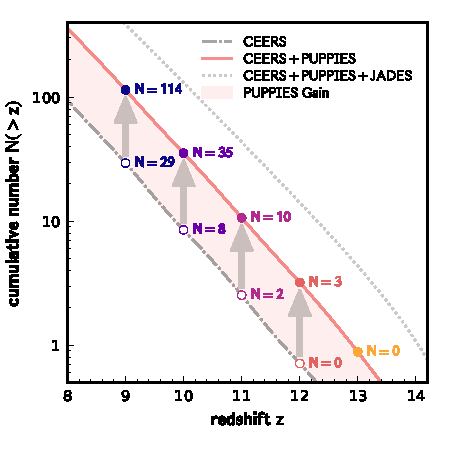
\includegraphics[width=0.6\textwidth]{figs/CN_surveys.pdf}
      \caption{\protect\rule{0ex}{5ex} The cumulative number of sources predicted to observeable to CEERS, PUPPIES, and JADES.}
      \vspace{-10mm}
\end{SCfigure}


\todo{What has been done and how will WAFLS change things?}
\todo{Should we mention Hubble constraints? - I feel we're not fighting Hubble but other Webb programmes.}

While the planned GTO/ERS programmes will begin the process of obtaining stronger constraints at $z>9$ the relatively small areas probed by these programs limits the number of bright galaxies. This limits our ability to constrain the bright-end of the LF, critical to characterise its overall shape. Compounding the small number of sources is the fact that these programmes, as predominantly contiguous surveys, will suffer from cosmic variance increasing the uncertainty on the number of galaxies by $\approx 1.5-2\times$ compared to the statistical uncertainty alone\cite{2020MNRAS.499.2401T}\cite{2020MNRAS.496..754B}\cite{2008ApJ...676..767T}. 

% \begin{SCfigure}
%     \includegraphics[width=0.6\textwidth]{figs/CV.pdf}
%       \caption{\protect\rule{0ex}{5ex} The predicted number of sources at $9<z<10$ as a function of F277W in CEERS, JADES, and WAFLS. The upper-panel shows the total variance $\sigma^2$ compared to the expected statistical variance $N$. This demonstrates that WAFLS suffers from minimal cosmic variance while both JADES and CEERS suffer a factor of $2-4$ larger variance than naively expected for the given number of galaxies.}
%       \label{fig:CV}
%       \vspace{-5mm}
% \end{SCfigure}

The wide area and pure parallel nature of WAFLS overcomes these issues. The WAFLS strategy is tuned to probe $M^{\star}$ ($M_{1500}=-20\ -\ 21$) galaxies at $9<z<11$ yielding roughly uniform number of galaxies per mag at F277W$27.5-29.5$ ($-21<M_{1500}<-18$) when combined with JADES and CEERS. Figure \ref{fig:CV} shows both the predicted number of sources and the total variance compared to the expected statistical variance for WAFLS, CEERS, and JADES. WAFLS yields not only $3\times$ as many galaxies as JADES+CEERS at F277W$<28.25$ but the resulting total uncertainty is virtually cosmic variance mitigated resulting in an even stronger gain. In Figure \ref{fig:LF} we show the resulting constraints on the $9.5<z<10.5$ LF from CEERS+JADES both with and without WAFLS. This highlights the strong improvement, particularly at $-21<M_{1500}<-20$ where $M^{\star}$ is expected to lie. The addition of WAFLS provides roughly uniform sampling of the LF over and reduces the uncertainty on both the parameters by around a factor of $2-3$. As shown in the right-hand panel WAFLS, when combined with CEERS and JADES, is able to discriminate between many current models. 

% \begin{figure}[h!]
%     \centering
%     \includegraphics[width=0.5\textwidth]{figs/LF_10_combined.pdf}
%     \includegraphics[width=0.45\textwidth]{figs/fitLF_alpha_phi.pdf}
%     \vspace{-5mm}
%     \caption{Expected constraints on the $9.5<z<10.5$ luminosity function, assuming the Mason+2015 model, for WAFLS, CEERS, and JADES. Uncertainties are corrected for the effects of cosmic variance. Sources are included if they are brighter than the 10$\sigma$ point-source limit. The right hand panel shows the joint constraints on the faint-end slope $\alpha$ and the number density at $M_{1500}=-20.5$ both using WAFLS and without WAFLS (JADES+CEERS). The right hand panel also shows various empirical and model predictions.}
%     \label{fig:LF}
% \end{figure}

\subsection*{The Physical Properties of Galaxies in the EoR}\label{sec:properties}




% THIS TEXT IS TAKEN FROM ANOTHER PROPOSAL IN PREP - IT SHARES SOME COIs SO I FEEL ITS FINE AS A REFERENCE

% 1.1: Physical Processes Regulating the Emergence of the First Galaxies
% The shape of the rest-frame UV luminosity function constrains the relative importance of the physical processes governing the conversion of gas into stars. These processes depends on numerous factors, including density, metallicity, magnetic field strength, turbulence, and a variety of feedback mechanisms. At the highest redshifts we have almost no empirical constraints on these processes, though theoretical predictions for galaxies in this era are beginning to emerge [e.g., 24, 16, 35, 39, 2]. However, these models use different prescriptions for the physics regulating the conversion of gas into stars, resulting in a wide range of predicted z > 10 luminosity functions. For example, Behroozi et al. [2] adopt an ansatz that galaxy specific SFRs (SFR per unit stellar mass) follow their halo’s specific mass accretion rate, reproducing the observed SFR density evolution at z <8. When extrapolated to even earlier times, it predicts a relatively shallow evolution at 8 < z < 15, with very bullish predictions for JWST surveys.
% Models that attempt to include the detailed physics of molecule formation, star forma- tion, and stellar feedback generally make more bearish predictions [e.g., 16, 35, 39], though their predictions differ dramatically at extreme redshifts (z > 8).
% Figure 2 shows the predicted UV luminosity functions from these models at z = 10 (top-
% middle) and z = 12 (top-right). At z =10 there are noticeable differences in the normalization (∆φ∗ ∼ 1 dex) and faint-end slope (∆α ∼ 0.5). This becomes even more evident at z = 12, where the models span ≥ 1 dex across all luminosities, leading to >∼2 dex variations in the normalization φ∗ and nearly 1 dex in the faint-end slope α. We show predictions for the constraints achievable with WDEEP (see Technical Justification for details), which begin to distinguish between these models at MUV = −17.5 (the ∼10σ limit at z =10).
% Why is there such disagreement in these models? As cosmological simulations can-
% not come close to resolving the formation of individual stars, they must assume many key
% physical relationships. Two in particular regulate the shape and normalization of the UV
% luminosity function at high redshift: the star-formation law (or star formation efficiency
% as a function of cold gas surface density), and the prescription for stellar feedback. Yung
% et al. [39] explored these physical processes using a semi-analytic model (SAM), exploring
% how modifications to these relationships altered the UV luminosity function, shown in the
% bottom panel of Figure 2. The purple shading shows the difference in luminosity func-
% tion predictions between assuming a linear relationship between molecular gas density and  ̇
% that SFRD scales as molecular gas density squared Σ∗ ∝ (ΣH2 )2 above a critical H2 surface density (upper envelope). These changes result in strong differences in the bright-end of the ̇UV luminosity function, where medium-depth wide-field programs such as CEERS will place constraints, but little change in the faint-end.

% However, Yung et al. [39] found that stellar feedback strongly influences star formation in low-mass halos, with significant changes in the predicted abundances of faint galaxies. They parameterized this with a stellar feedback relation slope (αrh) which characterizes the dependence of the mass loading factor of cold gas ejected by stellar feedback on the halo circular velocity. Yung et al. [39] found that changing αrh can change the number density of the lowest-mass observable galaxies (∼108M⊙; MUV ∼ −18 at z = 10) by up to 1 dex. The red shaded region in Figure 2 illustrates the range of luminosity function predictions from Yung et al. [39] when changing αrh = 2.0 (top) to 3.6 (bottom). The data points show the precision on the luminosity function measured by CEERS (green) and WDEEP (blue) for Yung et al’s fiducial model (αrh = 2.4). Our predicted WDEEP constraints have uncertainties which are ∼7× smaller than this range in models.
% By robustly identifying galaxies to m > 30, WDEEP will provide the first meaningful constraints on the stellar feedback physics in extremely early galaxies. Constraining the luminosity function to this precision will allow a robust determination of the observed SFR density to z = 12, distinguishing between the wide range of models shown in Figure 2. Finally, by constraining whether the SFR density evolves shallowly or steeply, WDEEP will provide significant constraints on models of reionization.

% As we discover galaxies closer and closer
% to the Big Bang, we will eventually wit-
% ness the periods during which galaxies
% have formed no more than a few gen-
% erations of stars, characterized by ex-
% tremely low metallicities. While pre-
% vious generations of simulations im-
% plied that discovering entire pockets
% of metal-free star-formation was possi-
% ble [so-called “Population III” galaxies;
% e.g. 32], more recent simulations pre-
% dict that Pop III star formation in early
% mini-halos at z ∼ 15–20 was likely very
% efficient at polluting the IGM with met-
% als, and so we might never expect to see
% metal-free star formation [e.g., 18, 17].
% The consequences for subsequent star-
% formation are critical — if all dense gas
% in the universe is rapidly enriched beyond the critical metallicity (Z ∼ 10−4 Z⊙), both the stellar initial mass function and stellar photospheric temperatures will likely not be dramat- ically different than that seen in low-metallicity environments in the early universe. If the opposite is true, and fairly massive metal-free stars can form down to even z ∼ 10, it will provide a distinct boost in the typical hardness of stellar spectra, with consequences on the ability of stellar light to reionize the IGM.
% Constraints on the typical metallicities of early galaxies are thus of intense interest. A straightforward measure of the physical properties of the stars is available via the UV spectral slope β; fλ ∝ λβ [9], which can be measured via broadband colors, with β < −3 a typical threshold for near-metal-free stellar populations. Observations with HST at z < 10 found no strong evidence for β < −2.5, thus the presently observable galaxies are consistent with somewhat low, but non-zero, metallicities, without much dust obscuration in the lowest mass galaxies [13, 10, 5, 34]. Our proposed NIRCam observations will measure four (three) rest-UV colors for galaxies at z ∼ 10 (12), allowing us to constrain the nature of their stellar populations. Simulations at our proposed depths show that with these multiple colors we can recover β with minimal bias and σβ = 0.2 to z > 13. Finally, our observations will improve measures of galaxies at z = 6–8, currently restricted to just one or two colors, measuring β with five colors.


\begin{SCfigure}
    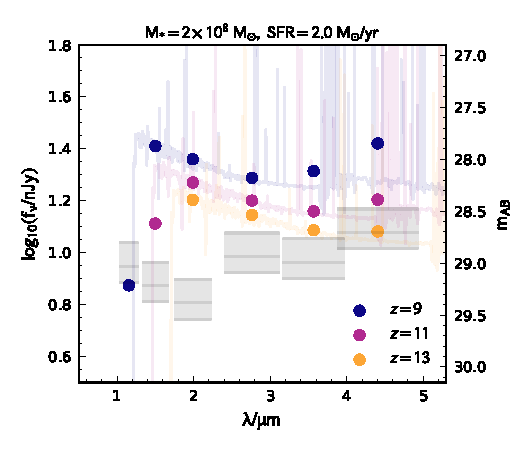
\includegraphics[width=0.6\textwidth]{figs/SED.pdf}
      \caption{\protect\rule{0ex}{10ex} The spectra and NIRCam fluxes of $5\times 10^{8}\ {\rm M_{\odot}}$ star forming galaxies at $z=9$ and $z=11$. Circled points denote a restricted 4 filter strategy; although this can be used to identify $z>9$ galaxies it neither enables the consistent measurement of the UV continuum slope $\beta$ across the target redshift range or allows constraints on the strength of the Balmer/$4000{\rm\AA}$ range.}
      \label{fig:SED}
\end{SCfigure}

The shape of the rest-frame UV continuum emission (the UV continuum slope, or $\beta$ where $f_{\lambda}\propto\lambda^{\beta}$) is a powerful probe of the physical properties of star forming galaxies. These properties include dust attenuation, stellar metallicity, star formation history, and ionising photon escape fraction \cite{2013MNRAS.430.2885W}. Particularly blue slopes ($\beta\simeq -3$) are indicative of the presence a young, low-metallicity, stellar population. While measurements of $\beta$ are available at $z\approx 7$ with {\em Hubble} these are typically measured with only a single colour over a relatively short wavelength baseline leading to large uncertainties and biases. While it is possible to measure $\beta$'s at $z\approx 10$ by combining {\em Hubble} and {\em Spitzer} observations \cite{2016MNRAS.455..659W}, these rely on the significantly shallower {\em Spitzer} imaging and have larger uncertainties. The 6 filter strategy of WAFLS (see Figure \ref{fig:SED}) will enable the consistent measurement of $\beta$ at $9<z<11$ over the entire rest-frame UV continuum. As demonstrated using simulated galaxies in Figure \ref{fig:beta}, when combined with F444W the degeneracy of $\beta$ with these physical properties can be broken allowing the measurement of stellar masses, specific star formation rates, and dust attenuation. Measuring the dust attenuation not only allows us to account for obscured star formation but will also help constrain the mechanism(s) responsible for the assembly of the large observed reservoirs of dust in the early Universe.



\begin{figure}[h!]
    \centering
    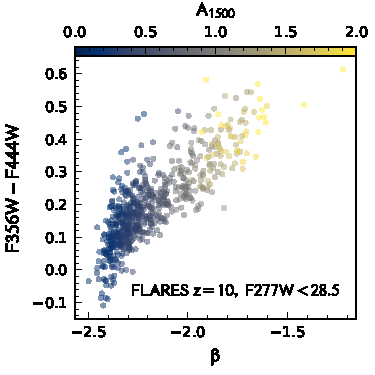
\includegraphics[width=0.3\textwidth]{figs/beta_A1500.pdf}
    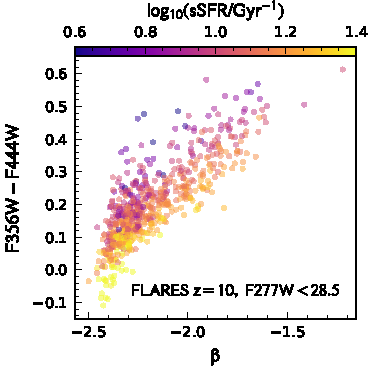
\includegraphics[width=0.3\textwidth]{figs/beta_sSFR.pdf}
    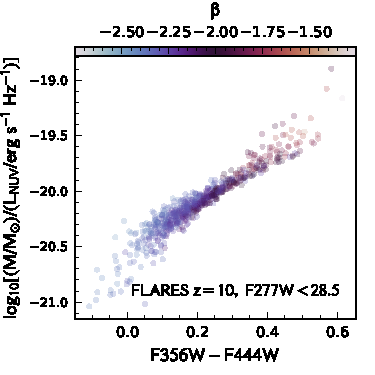
\includegraphics[width=0.3\textwidth]{figs/C_beta_MTOL.pdf}
    \caption{\emph{Left (middle):} The relationship between $\beta$ and F356W-F444W for simulated galaxies at $z=10$ colour-coded by $A_{1500}$ (sSFR) predicted by the FLARES simulation (Lovell+2020; Vijayan+2020). At these redshifts $\beta$ is strongly correlated with dust attenuation while at fixed $\beta$ the specific SFR is correlated with F356W-F444W. \emph{Right:} The relationship between F356W-F444W and the rest-frame NUV mass-to-light ratio. This demonstrates that stellar masses can be accurately determined using this single colour.}
    \label{fig:beta}
\end{figure}


% Morphologies

The morphologies and sizes of galaxies encode information about their structural properties and formation histories and are key observables that can be compared to galaxy formation models. Morphologies are also an important assumption used in the measurement of the luminosity function (reference) and only by simultaneously modelling the morphologies, redshifts, and fluxes is it possible to self-consistently measure the luminosity function and its uncertainties. Leveraging NIRCam's resolution WAFLS will provide sizes and morphologies of $9<z<11$ galaxies across the rest-frame UV ($0.1-0.4\mu$m). \todo{Maybe we should make a plot comparing the predicted size of galaxies to the NIRCam pixel scale and PSF?}




\subsection*{Legacy science}






%%%%%%%%%%%%%%%%%%%%%%%%%%%%%%%%%%%%%%%%%%%%%%%%%%%%%%%%%%%%%%%%%%%%%%%%%%%

%   2. TECHNICAL JUSTIFICATION
%       (see https://jwst-docs.stsci.edu/jwst-opportunities-and-policies/jwst-call-for-proposals-for-cycle-1/jwst-cycle-1-proposal-preparation)
%
%

\clearpage

\justifyobservations   % Do not delete this command.
% Enter your description of the observations.

\noindent
\underline{\bf Filter choice:} Simulations show that the combination of 3 filter pairs: {\bf F115W}, {\bf F150W}, {\bf F200W}, {\bf F277W}, {\bf F356W}, and {\bf F444W} is the optimum choice for \emph{robustly} identifying $z>9$ star forming galaxies. 2 pairs can in principle be used to detect galaxies $9<z<11$ however the contamination rate is higher and the accuracy/precision at $z>11$ drops significantly. 2 pairs also limits the extent to which the UV continuum slope $\beta$ can be measured \emph{consistently} across redshifts. Adding {\bf F090W} has little effect on the the reliability of the redshifts of galaxies at $z>9$ though does extend the redshift range down to $z\sim 7$ providing increased legacy science. While noting that 3 filter pair strategy best matches our scientific objectives these can be partially met or even \emph{exceeded} using a 2 or 4 pair strategy respectively. To keep PUPPIES as flexible as possible we can also make use of opportunities better suited to a 2 or 4 pair strategy though note a preference those opportunities amenable to our default scenario.

\todo{Photometric redshift tests}

\noindent
\underline{\bf Parallel opportunities:} PUPPIES is an opportunity led program: we are interested in obtaining deep NIRCam imaging in 10-20 independent pointings. Compared to a contiguous survey 10-20 independent sight-lines should reduce the cosmic variance (not total variance) by around $3-5$.

\noindent
To determine the type of opportunities that are available we use the public GTO and ERS APTs and filter out all observations already with attached coordinated parallels, with the \texttt{NoParallel} flag set, and those of targets with high-background ($>0.3\ $). For each target we then sum the science duration of all observations using the same instrument to obtain an approximate total science duration available to each valid target. The resulting predicted distribution of opportunities with science durations $t_{\rm SD}>10^{4}$ s is then shown in Figure \ref{fig:time_background}. This analysis suggests $\sim 50$ opportunities with $t_{\rm SD}>10^{4}$ s; assuming this distribution is representative of the final Cycle 1 observation suggests there should be $100-150$ useful opportunities.

\begin{SCfigure}
    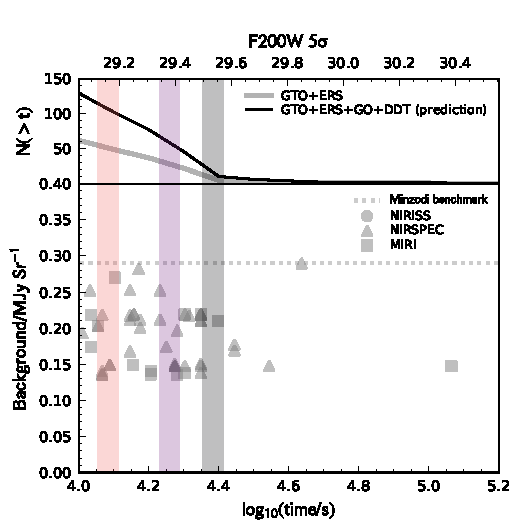
\includegraphics[width=0.6\textwidth]{figs/time_background.pdf}
      \caption{\protect\rule{0ex}{10ex} The predicted distribution of science durations $t_{\rm SD}$ and backgrounds for pure parallel observing opportunities based on the existing GTO and ERS programs. The vertical bands denote the 3 tiers used to define our fiducial survey while the horizontal lines denote the $2\mu$m \texttt{minzodi} benchmark background and the minimum background in several deep extragalactic fields. The top panel shows the resulting cumulative distribution of opportunities as well as an extrapolation to the full cycle 1 observations.}
      \label{fig:time_background}
\end{SCfigure}

\noindent
\underline{\bf Fiducial programme:}
Armed with this predicted we define a fiducial programme consisting of three tiers - ABC - assuming 4, 3, and 2 \texttt{deep8} 10 group exposures respectively. Reflecting the greater availability of shorter duration opportunities we choose, for this fiducial programme, to obtain 3, 5, and 10 pointings for the A, B, and C tiers respectively. The resulting area and depths achieved in each tier are summarised below. \textbf{The total exposure time as reported by the APT for the combination of the 3 tiers is 79.3 hours}.

\begin{table}[h!]
\begin{center}
\begin{tabular}{ |l|c|c|c|c|c|c|c|c| } 
\hline
\multicolumn{3}{|c|}{} & \multicolumn{6}{|c|}{$5\sigma$ point-source depth} \\
 \hline
Tier & $N_{p}$ & Area$/{\rm arcmin^2}$ & F115W & F150W & F200W & F277W & F356W & F444W \\
\hline
A & 3 & 27 & 29.19 & 29.37 & 29.54 & 29.09 & 29.15 & 28.86 \\
B & 5 & 45 & 29.03 & 29.22 & 29.38 & 28.94 & 28.99 & 28.70 \\
C & 10 & 91 & 28.81 & 28.99 & 29.16 & 28.71 & 28.77 & 28.48 \\
\hline
\end{tabular}
\end{center}
\vspace{-5mm}
\caption{The number of pointings $N_p$, area, and 5$\sigma$ point source depths in each filter for our 3 tiers for our fiducial survey.  Depths assume a short-wavelength (long-wavelength) apertures of $0.08$" ($0.16$"), background at the benchmark level of the \texttt{Minzodi} location as defined by \texttt{Pandeia}. The ABC tiers assume 4, 3, 2 exposures of 10 groups assuming the \texttt{DEEP8} readout mode respectively.}
\end{table}

\noindent
\underline{\bf Preferred distribution:} We would preferentially go deeper while keeping at least 10 independent sight-lines. 


\noindent
\underline{\bf Synergy with existing and planned surveys} PUPPIES will, partly through the expected availability of suitable parallel observing opportunities and partly through the primary scientific objectives, naturally complement planned programmes on \emph{Webb}, specifically CEERS and JADES. A comparison of the F150W, F200W, and F356W $5\sigma$ point-source depths and areas expected by WAFLS, CEERS, and JADES are shown in Figure \ref{fig:depth}. Figure \ref{fig:depth} also demonstrates the dramatic improvement of WAFLS over existing Hubble and Spitzer surveys. Compared to programmes reaching (surveying) a similar depth (area) on Hubble, WAFLS probes an approximately 10$\times$ larger area (1 magnitude deeper). There are no Spitzer surveys reaching a comparable depth in F356W/F444W with WAFLS reaching 2 magnitudes deeper than similar area surveys. By focusing on the $z>9$ Universe WAFLS will also complement the upcoming Euclid satellite which will be limited to $z\approx 8$. \todo{Needs updating}

\begin{SCfigure}
    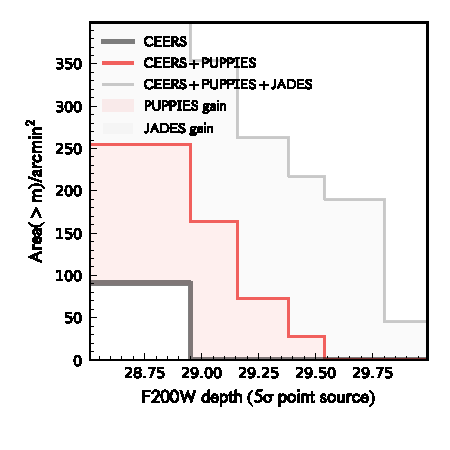
\includegraphics[width=0.6\textwidth]{figs/F200W.pdf}
      \caption{\protect\rule{0ex}{5ex} The cumulative area probed by WAFLS, JADES, CEERS, and existing \emph{Hubble} and \emph{Spitzer} surveys as a function of the H/F150W-band, F200W, and $3.6\mu$m/F356W (right) depths. \todo{Which is better?}}
      \label{fig:depth}
\end{SCfigure}


\noindent
\underline{\bf Additional constraints} When selecting potential parallel slots we will not only consider potential science duration and background but also the availability of ancillary observations and accessibility to other facilities (e.g. ALMA).



%%%%%%%%%%%%%%%%%%%%%%%%%%%%%%%%%%%%%%%%%%%%%%%%%%%%%%%%%%%%%%%%%%%%%%%%%%%

%   3. SPECIAL REQUIREMENTS
%        (see https://jwst-docs.stsci.edu/jwst-opportunities-and-policies/jwst-call-for-proposals-for-cycle-1/jwst-cycle-1-proposal-preparation)
%
%
\specialreq             % Do not delete this command.
% Justify your special requirements here, if any.

%%%%%%%%%%%%%%%%%%%%%%%%%%%%%%%%%%%%%%%%%%%%%%%%%%%%%%%%%%%%%%%%%%%%%%%%%%%

%   4. COORDINATED PARALLEL OBSERVATIONS
%        (see https://jwst-docs.stsci.edu/jwst-opportunities-and-policies/jwst-call-for-proposals-for-cycle-1/jwst-cycle-1-proposal-preparation)
%
%
\coordinatedobs % Do not delete this command.
% Enter your coordinated parallel observing plans here, if any.

%%%%%%%%%%%%%%%%%%%%%%%%%%%%%%%%%%%%%%%%%%%%%%%%%%%%%%%%%%%%%%%%%%%%%%%%%%%

%   5. JUSTIFY DUPLICATIONS
%        (see https://jwst-docs.stsci.edu/jwst-opportunities-and-policies/jwst-call-for-proposals-for-cycle-1/jwst-cycle-1-proposal-preparation)
%
%
\duplications           % Do not delete this command.
% Enter your duplication justifications here, if any.

%%%%%%%%%%%%%%%%%%%%%%%%%%%%%%%%%%%%%%%%%%%%%%%%%%%%%%%%%%%%%%%%%%%%%%%%%%%

%   6. ANALYSIS PLAN
%       (see https://jwst-docs.stsci.edu/jwst-opportunities-and-policies/jwst-call-for-proposals-for-cycle-1/jwst-cycle-1-proposal-preparation)
%
%
\analysisplan % Do not delete this command.
% Describe the data processing and analysis plan here.

%%%%%%%%%%%%%%%%%%%%%%%%%%%%%%%%%%%%%%%%%%%%%%%%%%%%%%%%%%%%%%%%%%%%%%%%%%%

\clearpage

\bibliography{WAFLS,WAFLS_quiescent}


\end{document}          % End of proposal. Do not delete this line.
                        % Everything after this command is ignored.
